% THIS TEMPLATE IS A WORK IN PROGRESS
% Adapted from an original template by faculty at Reykjavik University, Iceland

\documentclass{scrartcl}

% Adapted from an original template by Hlyni Arnórssyni, Reykjavik University, Iceland
%
% ------------------------------ SETTINGS
\usepackage{geometry}

\geometry{
	paper=a4paper, % Paper size
	top=2.5cm, % Top margin
	bottom=2.5cm, % Bottom margin
	left=2.5cm, % Left margin
	right=2.4cm, % Right margin
	headheight=0.75cm, % Header height
	footskip=1.5cm, % Space from the bottom margin to the baseline of the footer
	headsep=0.75cm, % Space from the top margin to the baseline of the header
	%showframe, % Uncomment to show how the type block is set on the page
}

\usepackage{blindtext}
%-------------------------------- Character encoding ----------------------------
\usepackage[T1]{fontenc}
\usepackage[utf8]{inputenc}

%----------------------------- Mathematics packages from AMS ---------------

\usepackage{amsmath, amsfonts, amsthm, amssymb}
\usepackage{braket, nicefrac}

% ----------- International System of Units
\usepackage{siunitx}

%------------------------------ Lists / numbers -------------------------
\usepackage{enumitem, multicol}

%------------------------------- Figure insertions --------------
\usepackage{graphicx, float}  % Use option [H] to force the placement of a figure
\usepackage{keystroke}
\usepackage{pgfplots}\usepgfplotslibrary{units}\pgfplotsset{compat=1.16}

%------------------------------- Line Spacing --------------
\usepackage{setspace}

%------------------------------- Depth of the ToC --------------
\setcounter{tocdepth}{2}

%%%%%%%%%%%%%%%%%%%%%%%%%% Hyperlink References %%%%%%%%%%%%%%%%%%%%%%%%%%%
\usepackage{hyperref}

%--------------------% Storage Path for images %-----------------%
\graphicspath{{graphics/}{Graphics/}{./}{./research-paper/capstone/capstone/Graphics}}

%%%%%%%%%%%%%%%%%%%%%%%%%% Environments %%%%%%%%%%%%%%%%%%%%%%%%%%%
\renewenvironment{abstract}{
    \begin{center}
    \textbf{Abstract}
    \vspace{0.5cm}
    \par\itshape
    \begin{minipage}{0.8\linewidth}}{\end{minipage}
    \noindent\ignorespaces
    \end{center}
}

\newenvironment{keywords}{
    \begin{center}
    \textbf{Keywords}
    \vspace{0.5cm}
    \par
    \begin{minipage}{0.8\linewidth}}{\end{minipage}
    \noindent\ignorespaces
    \end{center}
}

\newenvironment{preface}{
    \begin{center}
    \textbf{Preface}
    \vspace{0.5cm}
    \par
    \begin{minipage}{0.8\linewidth}}{\end{minipage}
    \noindent\ignorespaces
    \end{center}
}

\newenvironment{acknowledgements}{
    \begin{center}
    \textbf{Acknowledgements}
    \vspace{0.5cm}
    \par
    \begin{minipage}{0.8\linewidth}}{\end{minipage}
    \noindent\ignorespaces
    \end{center}
}

\hbadness=10000

 


\begin{document}
%Title of the report, name of coworkers and dates (of experiment and of report).
\begin{titlepage}
	\centering
	
\includegraphics[width=0.6\textwidth]{nyush-logo.jpeg}\par
	\vspace{2cm}
	%%%% COMMENT OUT irrelevant lines among the 3 below
  {\scshape\LARGE Computer Science, Data Science \& \par}  %if you're a CS major
  {\scshape\LARGE Computer Systems Engineering \par}
	\vspace{1cm}
	{\scshape\Large Capstone Report - Fall 2024\par}
	%{\large \today\par}
	\vfill
	
	%%%% PROJECT TITLE
	{\huge\bfseries Benchmarking ZK Virtual Machines for Privacy-Preserving Machine Learning Applications\par}
	\vfill
	
	%%%% AUTHOR(S)
	{\Large\itshape Lawrence Lim\\ Siddhartha Tuladhar\\ Brandon Gao\\}\par
	\vspace{1.5cm}

	\vfill
	supervised by\par
	%%%% SUPERVISOR(S)
  Promethee Spathis

	\vfill
% Bottom of the page
\end{titlepage}

\newpage

\begin{preface}
 As a team comprising a Computer Systems Engineering major, a Computer Science major, and a Data Science major, we bring diverse perspectives and expertise to address the complex challenges at the intersection of privacy, security, and scalability in technology. This project was inspired by the increasing importance of privacy-preserving computation, particularly in sensitive fields like finance, where secure data handling is paramount. Our collective academic backgrounds have allowed us to explore innovative approaches to these challenges, drawing from distributed systems, cryptography, and data analytics.

Our target audience includes researchers, developers, and industry professionals who are advancing privacy technologies, blockchain systems, and secure data frameworks. By benchmarking zero-knowledge virtual machines (zkVMs) in the context of financial data, this project seeks to provide valuable insights into their capabilities and limitations, contributing to the ongoing development of secure and privacy-centric computational tools.       
\end{preface}

\vspace{1cm}

\begin{acknowledgements}
We sincerely thank our advisor, Professor Promethee Spathis, for their guidance and support throughout this project. We are also grateful to the Professor Benedikt Bunz for providing the initial ideation for this project. Lastly, we are grateful to our families and friends for their encouragement and support.\end{acknowledgements}

\newpage

\begin{abstract}
This work addresses the challenge of securely processing sensitive data in privacy-critical applications like finance. Zero-knowledge virtual machines (zkVMs) offer a promising solution, but face issues with complexity and proof generation time. We benchmark three zkVMs—SP1, Jolt, and RISC-0—by training a ridge regression model on financial data, evaluating their performance and identifying key bottlenecks. Our findings highlight zkVMs’ potential for privacy-preserving computation and provide insights for improving their practical adoption.
\end{abstract}
\vspace{1cm}

\begin{keywords}
\centering
         \textbf{Capstone; Computer science; Machine Learning; Zero-Knowledge Proofs, Zero-Knowledge Virtual Machines, Jolt, SP1, Risc0, NYU Shanghai}
\end{keywords}

\newpage



\doublespacing
\tableofcontents
\singlespacing

\newpage

\doublespacing

\section{Introduction}

Your introduction briefly explains the problem you address, and what you've achieved towards solving the problem. It's an edited and updated version of your context and objectives from your topic outline document.

\subsection{Context}

Currently, there exists a large amount of sensitive customer data that is extremely valuable but not being monetized to its fullest extent due to a combination of compliance and ethical concerns. An essential category of this data is personal financial data. Due to the sensitive nature of this data and strict compliance laws, current Fintech platforms require users’ explicit permission to access sensitive information like credit history, transaction history, and income. However, \textbf{Zero Knowledge Proof (ZKP)} can be utilized to develop services and algorithms that utilize the sensitive data without explicitly revealing it. A ZKP is a cryptographic method of proving a statement is true without revealing any other information besides the fact that the statement is true. ZKPs have three fundamental characteristics:

\begin{itemize}
    \item \textbf{Completeness:} If a statement is true, an honest prover can prove to an honest verifier that they have knowledge of the correct input.
    \item \textbf{Soundness:} If a statement is false, a dishonest prover is unable to convince an honest verifier that they have knowledge of the correct input.
    \item \textbf{Zero-knowledge:} No other information about the input is revealed to the verifier from the prover besides the fact that the statement is true.
\end{itemize}

Currently, the most-friendly way of generating a ZKP is through the use of zero-knowledge virtual machines (zkVMs). A zkVM, is simply a VM implemented as a circuit for a ZKP system. So, instead of proving the execution of a program, as one would normally do in ZKP systems, you prove the execution of the bytecode of a given Instruction Set Architecture (ISA). However, the zkVM landscape is in early development, and proof generation is bottlenecked by the complexity of the program and hardware limitations. In this paper, we provide a quantatitve and qualitative analysis on the current state of zkVMs on a real-world use case by generating a proof of a machine learning (ML) algorithm on dummy financial data.

\subsection{Objective}

The objective of this paper is to provide researchers, developers, and industry professionals a comprehensive review on utilizing zkVMs in a real-world use case. In order to achieve this, we benchmark SP1\cite{Roy2024}, Risc0\cite{bruestle2023risc}, and Jolt\cite{arun2024jolt}, since they all compile to RISC-V, which is an extremely popular compile target for most programming languages (Rust, C++, LLVM). We provide a quantative analysis on proof generation time and proof verification time. Additionally, we provide a qualitative analysis on the developer experience on developing ML algorithms for these zkVMs. The ML algorithm that we use is the ridge regression model. 

\section{Related Work}

Your related work section positions your problem and your approach with respect to other, maybe similar, projects you've found in the literature.
It "\textit{should not only explain what research others have done, but in each case should compare and contrast that to your work and also to other related work. After reading this section, a reader should understand the key idea and contribution of each significant piece of related work, how they fit together, and how your work differs.}"\footnote{\href{https://homes.cs.washington.edu/~mernst/advice/write-technical-paper.html\#related-work}{Michael Ernst - How to write a technical paper}} 
%%%% DO NOT write a related work section that is just a laundry list of other papers, with a sentence about each one that was lifted from its abstract, and without any critical analysis nor deep comparison to other work.

It's an edited and updated version of your literature review. Here are a few examples of how to insert citations like~\cite{Groth2016}, \cite{Roy2024}, and also~\cite{goldreich1991proofs}, or even~\cite{arun2024jolt}

\subsection{Cryptographic Protocols and Foundational Theories}

Groth’s\cite{Groth2016} seminal work on pairing-based non-interactive arguments contributed to reducing the size and complexity of ZKPs, providing the foundation for more practical implementations in cryptographic systems. By focusing on optimizing the size of non-interactive zero-knowledge proofs (NIZKs), this research addressed a core challenge in making ZKPs scalable and suitable for real-world applications. Similarly, the foundational paper by Goldreich et al.\cite{goldreich1991proofs} established the theoretical basis for zero-knowledge proofs, demonstrating that all nondeterministic polynomial (NP) problems can be proven without revealing anything beyond their validity. Both of these lay the groundwork for subsequent developments in the field, making it possible to use ZKPs across diverse cryptographic applications.
In more recent works, Ben-Sasson et al.\cite{ben2018scalable} introduced a ZKP system that ensures computational integrity while being both scalable and post-quantum secure. This system is designed to be transparent, avoiding the need for a trusted setup, and addresses the growing concern of quantum security in cryptographic protocols. The focus on transparency and scalability ties this work to Groth’s research but extends it by addressing future-proofing for quantum security. Ben-Sasson et al.\cite{ben2019aurora} further contributed to the field with Aurora, a ZKP system that provides transparent succinct arguments for Rank-1 Constraint Systems (R1CS), which are essential in blockchain applications. Like the earlier work, Aurora emphasizes transparency without a trusted setup but narrows its application to constraint systems, making it more suitable for decentralized verification in blockchain environments.

\subsection{Virtual Machine-based ZK Systems}

ZKPs have also found a significant place in virtual machine environments, where proof efficiency and verification times are critical. Arun et al.\cite{arun2024jolt} present Jolt, a zero-knowledge Succinct Non-Interactive Argument of Knowledge (zkSNARK) system optimized for virtual machines (VMs), which uses a new lookup technique to reduce proof size and verification time. This optimization makes Jolt effective in environments where complex computations occur, and proof generation must remain efficient. In comparison, Bruestle and Gafni\cite{bruestle2023risc} introduced the RISC-0 zkVM, a system designed to produce scalable, transparent proofs for computations based on the RISC-V instruction set. While both Jolt and RISC Zero address proof generation in VMs, RISC Zero focuses more on architecture-specific applications, such as the RISC-V ecosystem, which contrasts with Jolt’s broader application to virtual machines. RISC Zero’s Zeth system\cite{risc2023zeth} pushes the boundaries of ZKP applications in blockchain by drastically reducing the time required to prove Ethereum blocks, shifting from hours to minutes. Zeth’s optimization specifically targets blockchain verification, offering practical advantages for consensus mechanisms. When compared with Jolt and RISC-0, Zeth is specialized for blockchain environments, whereas the former systems focus on more general-purpose proof generation within virtual machines.

\subsection{Machine Learning in ZKPs}

Machine Learning is a In Wang et al. s study, the authors developed an efficient ZKP-based pipeline for classical machine learning inference, focusing on privacy-preserving inference that ensures model accuracy without exposing sensitive model information. This system optimizes zero-knowledge inference, making it highly applicable to real-world ML applications where data privacy is paramount. Similarly, [8] Sathe et al. (n.d.) provided a comprehensive survey of ZKP applications in machine learning, covering a range of cryptographic techniques and their applicability to neural networks, decision trees, and other ML models. Their survey offers a broader comparison of ZKP techniques in the ML space, providing essential context for more specific systems like that of Wang et al.
Lastly, [9] Ganescu and Passerat-Palmbach (2024) extended the application of ZKPs to generative AI models, by proposing a system that enhances trust in AI by allowing for the verification of generative models without exposing underlying data. This application is critical in AI-driven environments where sensitive inputs and outputs must be safeguarded while still proving the model’s validity.

\section{Solution}

The solution section covers all of your contributions (architecture, algorithms, formulas, findings).
It explains in detail each contribution, if possible with figures/schematics.

Don't forget that a figure goes a long way towards helping your reader understand your work. For instance, Figure~\ref{fig:ascent} outlines the layers involved in a distributed certification service, and how they articulate together. Nevertheless, a figure must always come with at least one paragraph of explanation. The rule is that anyone should be able to understand your solution from reading the text in this section, even if they skip the figures.

\begin{figure}[H]
	\begin{center}
		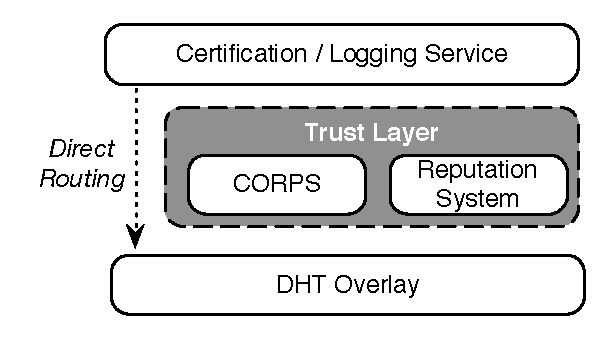
\includegraphics[scale=0.7]{ascent-archi.pdf}
	\end{center}
	\caption{Architecture of our distributed certification service}
	\label{fig:ascent}
\end{figure}

Figure~\ref{fig:log-archi} is a pretty good example of a figure that is completely useless unless it is not accompanied by a textual explanation.

\begin{figure}
	\begin{center}
		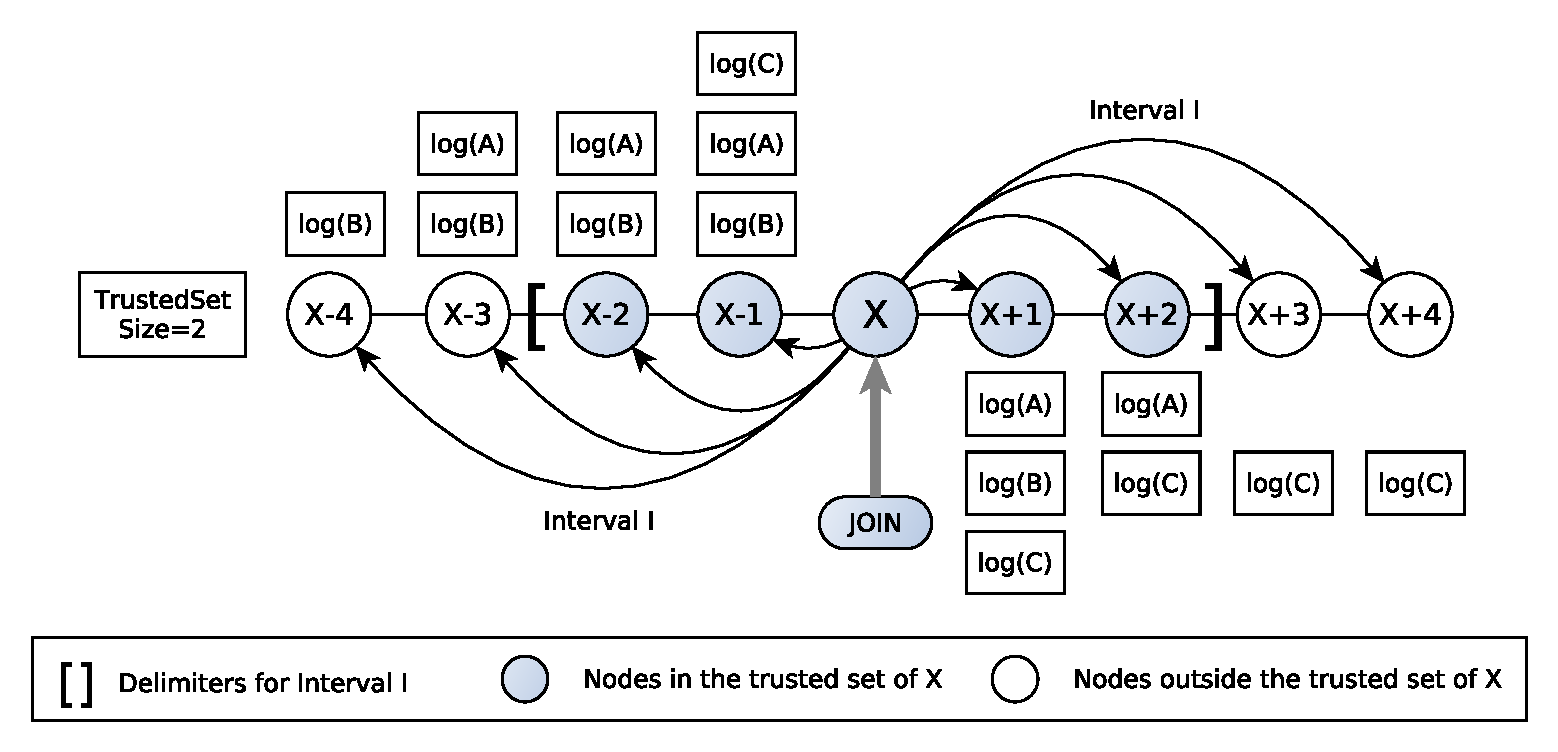
\includegraphics[scale=0.5]{certificates-log-archi.pdf}
	\end{center}
	\caption{Try to guess what this figure illustrates; I double-dare you...}
	\label{fig:log-archi}
\end{figure}



\section{Results and Discussion}

The results section details your metrics and experiments for the assessment of your solution. It then provides experimental validation for your approach with visual aids such as data tables and graphs. In particular, it allows you to compare your idea with other approaches you've tested, for example solutions you've mentioned in your related work section.

\subsection{Experimentation protocol}

It is of the utmost importance to describe how you came up with the measurements and results that support your evaluation.

\subsection{Data tables}

Every data table should be numbered, have a brief description as its title, and specify the units used. 

As an example, Table~\ref{tab:my_label} compares the average latencies of native application calls to networked services. The experiments were conducted on an Apple MacBook Air 2010 with a CPU speed of 1.4GHz and a bus speed of 800MHz. Each data point is a mean over 20 instances of each call, after discarding both the lowest and the highest measurement.

\begin{table}[ht]
    \centering
    \begin{tabular}{llr}
\hline
\multicolumn{2}{c}{Network Applications} \\
\cline{1-2}
Service    & Protocol & Latency (\si{\ms}) \\
\hline
DNS         & UDP       & \SI{13.65}{\ms}      \\
            & TCP       & \SI{0.01}{\ms}       \\
NTP         & UDP       & \SI{92.50}{\ms}      \\
SMTP        & TCP       & \SI{33.33}{\ms}      \\
HTTP        & TCP       & \SI{8.99}{\ms}       \\
\hline
\end{tabular}
    \caption{Comparison of latencies between services running on \texttt{localhost}.}
    \label{tab:my_label}
\end{table}

\subsection{Graphs}

Graphs are often the most important information in your report; you should design and plot them with great care. A graph contains a lot of information in a short space. Graphs should be numbered and have a title. Their axes should be labelled, with the quantities and units specified. Make sure that individual data points (your measurements) stand out clearly. And of course, always associate your graph with text that explains your results, and outlines the conclusions you draw from these results.

\begin{figure}
	\begin{center}
		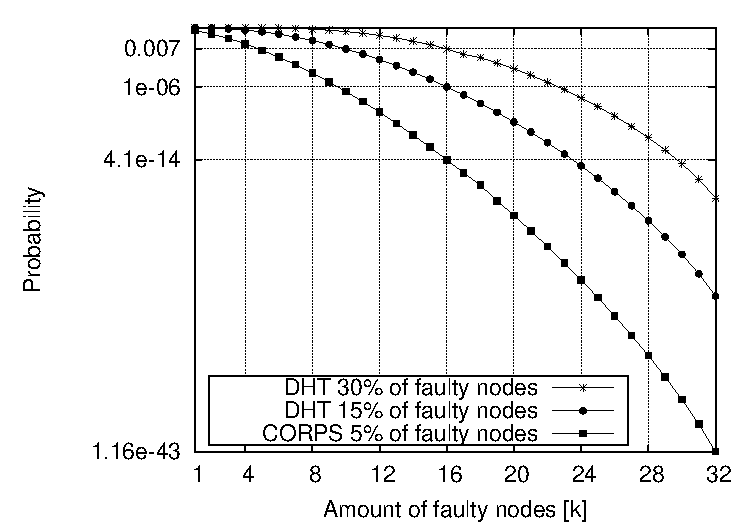
\includegraphics[scale=0.9]{perf-plot-1.pdf}
	\end{center}
	\caption{Probability of including [k] faulty/malicious nodes in the service}
	\label{graph:faulty-proportion-plot}
\end{figure}

For example, Figure~\ref{graph:faulty-proportion-plot} compares the efficiency of three different service architectures in eliminating adversarial behaviors. Every data point gives the probability that $k$ faulty/malicious nodes managed to participate in a computation that involves 32 nodes. In the absence of at least one reliable node ($k = 32$), the failure will go undetected ; but the results show that this case is extremely unlikely, regardless of the architecture. The most significant result pertains to $k = 16$: the reliable nodes detect the failure, but cannot reach a majority to recover. The graph shows that the \texttt{CORPS 5\%} architecture is much more resilient than the \texttt{DHT 30\%} architecture, by a magnitude of $10^{11}$.


\section{Discussion}
The discussion section focuses on the main challenges/issues you had to overcome during the project. Outline what your approach does better than the ones you mentioned in your related work, and explain why. Do the same with issues where other solutions  outperform your own. Are there limitations to your approach? If so, what would you recommend towards removing/mitigating them? Given the experience you've gathered working on this project, are there other approaches that you feel are worth exploring?

\section{Conclusion}

Give a clear, short, and informative summary of all your important results. Answer the initial question(s) or respond to what you wanted to do, as stated in your introduction. It can be a short table or a list, and possibly one or two short comments or explanations. 

Target a reader who may not have time to read the whole report yet, but needs the results or the conclusions immediately. This is a typical situation in real life. Some readers will read your introduction and skip to your conclusion first, and read the whole report only later (if at all).

You may also draw perspectives. What's missing? In what directions could your work be extended?

\newpage
\singlespacing
\bibliographystyle{IEEEtran}
\bibliography{references}


%------ To create Appendix with additional stuff -------%
%\newpage
%\appendix
%\section{Appendix}
%Put data files, CAD drawings, additional sketches, etc.

\end{document}
 
